\documentclass[handout]{beamer}

\usetheme[progressbar=frametitle]{metropolis}
\metroset{block=fill}

\subtitle{NTIN071 Automata and Grammars}
\author{Jakub Bulín (KTIML MFF UK)}

\date{Spring 2025\\ 
    \vspace{1in} 
    \begin{flushleft}
        \it \footnotesize * Adapted from the Czech-lecture slides by Marta Vomlelová with gratitude. The translation, some modifications, and all errors are mine.
    \end{flushleft}
}

%% packages

\usepackage{amsmath}
\usepackage{amssymb}
\usepackage{amsthm}
\usepackage{cancel}
\usepackage{color}
\usepackage{colortbl}
\usepackage{forest}
\usepackage[utf8x]{inputenc}
\usepackage{multicol}
\usepackage{multirow}

%% colors
\definecolor{Gray}{gray}{0.9}

%% TikZ
\usepackage{tikz}
    \usetikzlibrary{
        automata,
        arrows,
        backgrounds,
        decorations.pathmorphing,
        fit,
        positioning,
        shapes,
        shapes.geometric,
        tikzmark
    } 
    \tikzset{>=stealth',shorten >=1pt,auto,node distance=2cm}
    \tikzset{initial text={}}
    \tikzset{elliptic state/.style={draw,ellipse}}

%% amsthm
\theoremstyle{plain}
    \newtheorem*{algorithm}{Algorithm}    
    \newtheorem*{observation}{Observation}
    \newtheorem*{proposition}{Proposition}

\theoremstyle{remark}
    \newtheorem*{exercise}{Exercise}
    \newtheorem*{remark}{Remark}

%% macros
\DeclareMathOperator{\RegE}{RegE}
\DeclareMathOperator{\RL}{RL}

% Just for Lecture 2
\newcommand{\x}{$\times$}
\newcommand{\nx}{\ }



\title{Lecture 10 -- Turing Machines}


\begin{document}


\frame{\titlepage}


\begin{frame}{Recap of Lecture 9}
	
    \begin{itemize}        
        \item Closure properties of context-free languages (including substitution, homomorphism, inverse homomorphism)
        \item Also closure properties of deterministic CFLs
        \item Dyck languages, a characterization of context-free languages
    \end{itemize}
	
\end{frame}


\section{\sc Chapter 3: Turing Machines}


\section{3.1 Turing machine}


\begin{frame}{History and motivation}
    
    1931--1936 Gödel, Church, Turing, Kleene: formalize \alert{`algorithms'}
    
    \smallskip
    
    \alert{Turing machine}: a general model of any computer
    \begin{itemize}
        \item a two-way infinite \alert{tape} (sequential memory)
        \item a \alert{head} to read/write, moves in both directions
        \item a control unit (finite state)
    \end{itemize}
    \vspace{-9pt}
    \begin{center}
        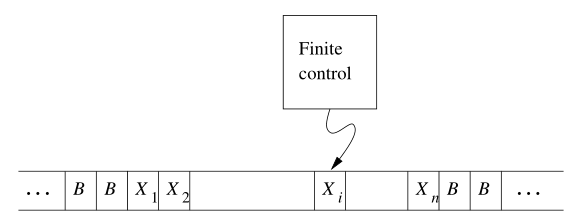
\includegraphics[width=0.8\textwidth]{files/tm1.PNG}  
    \end{center}        
    \vspace{-9pt}
    Other formalizations: RAM, $\lambda$-calculus, partially recursive functions

    \alert{Computability theory}: what problems can['t] computers solve?

\end{frame}


\begin{frame}{The definition}

    A \alert{Turing Machine (TM)} is $M=(Q,\Sigma,\Gamma,\delta,q_0,B,F)$ where:
    
    \begin{itemize}
        \item $Q$ is a finite, nonempty set of \alert{states}
        \item $\Sigma$ is a finite, nonempty \alert{input alphabet} 
        \item $\Gamma$ is a finite, nonempty \alert{tape alphabet}, $\Gamma \supseteq \Sigma$, $Q\cap \Gamma=\emptyset$
        \item $\delta\colon(Q\setminus F)\times\Gamma\rightarrow Q\times \Gamma\times \{L,R\}$ is the (partial) \alert{transition function}, i.e., one instruction is $\delta(q,x)=(p,Y,D)$ where:
        \begin{itemize}
            \item $q\in Q\setminus F$ is the current state [no transitions out of final states]
            \item $X\in\Gamma$ is the tape symbol in the current cell
            \item $p\in Q$ is the next state to switch to
            \item $Y\in \Gamma$ is the tape symbol to rewrite $X$ with in the current cell
            \item $D\in \{L,R\}$ is the \alert{direction} in which the head then moves
        \end{itemize}
        \item $q_0\in Q$ is the \alert{start state}
        \item $B\in\Gamma\setminus\Sigma$ is the \alert{blank symbol}, initially written in all but finitely many cells that hold the input symbols
        \item $F\subseteq Q$ are the \alert{final} or \alert{accepting} states
    \end{itemize}

\end{frame}


\begin{frame}{Describing computation: configurations}

    \textbf{Recall} \alert{computation graph}: vertices=\alert{configurations}, arcs=\alert{moves}~$\vdash$


    A \alert{configuration} of a TM is a finite string 
    $$
    X_1X_2\ldots X_{i-1}qX_iX_{i+1}\ldots X_n
    $$

    \begin{itemize}
        \item $q\in Q$ is the current state
        \item $X_1\ldots X_n\in\Gamma^*$ describe the contents of the relevant portion of the tape, that is, between
        \begin{itemize}
            \item the first (leftmost) non-blank symbol or head position, and
            \item the last (rightmost) non-blank symbol or head position
        \end{itemize} 
        \item the tape head is scanning the $i$-th symbol $X_i\in\Gamma$
    \end{itemize}
    
\end{frame}


\begin{frame}{Describing computation: moves}

    For \alert{moves} of a TM $M$, use same notation as for PDA: $\vdash_M, \vdash_M^*, \vdash^*$
    
    \medskip

    \begin{itemize}
        \item For $\delta(q,X_i)=(p,Y,L)$: 
        $$
        X_1X_2\ldots X_{i-1}qX_iX_{i+1}\ldots X_n \vdash_M X_1X_2\ldots X_{i-2}pX_{i-1}\textbf{Y}X_{i+1}\ldots X_n
        $$
        \item For $\delta(q,X_i)=(p,Y,R)$: 
        $$
        X_1X_2\ldots X_{i-1}qX_iX_{i+1}\ldots X_n \vdash_M X_1X_2\ldots X_{i-1}\textbf{Y}pX_{i+1}\ldots X_n
        $$
    \end{itemize}

    \medskip

    And $\vdash_M^*$ is a reflexive, transitive closure of $\vdash_M$ (oriented \alert{path} in the computation graph).

    \medskip

    \alert{initial configuration:} $q_0w$ for the input word $w\in\Sigma^*$\\
    \alert{accepting configurations:} those where $q\in F$, any tape contents (i.e., in our definition, the TM doesn't need to `clean' the tape)

\end{frame}


\begin{frame}{The language, an example}

    The language \alert{recognized by} a TM $M=(Q,\Sigma, \Gamma, \delta,q_0,B,F)$ is:    
    $$
    \alert{L(M)}=\{w\in \Sigma^*\mid q_0w \vdash_M^* \alpha p \beta, p\in F, \alpha,\beta \in \Gamma^*\}
    $$
    A language is \alert{recursively enumerable} if it is recognized by some TM

    \bigskip

    \begin{example}
        The following TM accepts the language $L=\{0^n1^n\mid n\geq 1\}$:
        $$
        M=(\{q_0,q_1,q_2,q_3,q_4\},\{0,1\},\{0,1,X,Y,B\},\delta,q_0,B,\{q_4\})
        $$

        \vspace{-15pt}
        \begin{center}
            \small
            \begin{tabular}{c | c c c c c}
            $\delta$ & $0$ & $1$ & $X$ & $Y$ & $B$\\
            \hline \hline
            $q_0$ & $(q_1,X,R)$& -- & -- & $(q_3,Y,R)$& --\\
            $q_1$ & $(q_1,0,R)$& $(q_2,Y,L)$& -- & $(q_1,Y,R)$& --\\
            $q_2$ & $(q_2,0,L)$& -- & $(q_0,X,R)$& $(q_2,Y,L)$& --\\
            $q_3$ & -- & -- & -- & $(q_3,Y,R)$& $(q_4,B,R)$\\
            $q_4$ & -- & -- & -- & -- & --
            \end{tabular}
        \end{center}
        \vspace{-9pt}
    \end{example}

\end{frame}


\begin{frame}{Transition diagram}

    \vspace{-6pt}
    \alert{nodes} are states, \alert{arcs} $q\to p$ are labeled by $X/YD$ for all $\delta(q,X)=(p,Y,D)$ (use $D\in\{\leftarrow,\rightarrow\}$ instead of $\{L,R\}$)
    
    \vspace{-3pt}
    \begin{center}
        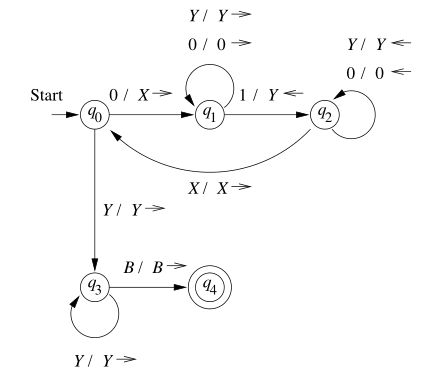
\includegraphics[width=0.72\textwidth]{files/tmTrans.PNG}
    \end{center}
    
\end{frame}


\begin{frame}{The program explained}

    \vspace{-6pt}
    \begin{multicols}{2}
        Recognizes \alert{$L=\{0^n1^n\mid n>0\}$}.

        \vspace{12pt}

        On tape always $X^*0^*Y^*1^*$.

        \vspace{12pt}

        Repeatedly rewrite a $0$ to $X$, and the corresponding $1$ to $Y$:

        \begin{center}
            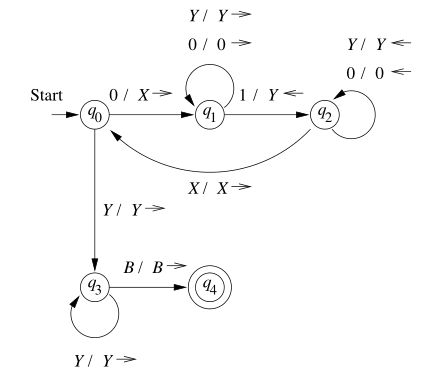
\includegraphics[width=0.45\textwidth]{files/tmTrans.PNG}
        \end{center}

    \end{multicols}   
    
    \vspace{-1.25cm}

    \begin{itemize}
        \item[$q_0$:] rewrite $0$ to $X$, switch to $q_1$
        \item[$q_1$:] search forward for the first $1$, rewrite to $Y$, switch to $q_2$
        \item[$q_2$:] search backward for the last $X$, go forward, switch to $q_0$
    \end{itemize}

    If $q_0$ sees $0$, continue as above, if it sees $Y$, switch to $q_3$    
    \begin{itemize}
        \item[$q_3$:] moves to the end to check that there are no remaining $1$s
        \item if $q_3$ finds $B$, switch to $q_4$, accept (accepting state)
        \item if $q_3$ finds $1$, fail (no instruction, not accepting state) 
    \end{itemize}

\end{frame}


\begin{frame}{Computation examples: $w=\alert{0011}$ and $w=\alert{0010}$}
    
    \small

    \begin{columns}

        \column{0.5\textwidth}

        \vspace{-0.75cm}
        \begin{align*}
            q_0\alert{0011}&\vdash\\
            Xq_1011&\vdash\\
            X0q_111&\vdash\\
            Xq_20Y1&\vdash\\
            q_2X0Y1&\vdash\\
            Xq_00Y1&\vdash\\
            XXq_1Y1&\vdash\\    
            XXYq_11&\vdash\\
            XXq_2YY&\vdash\\
            Xq_2XYY&\vdash\\
            XXq_0YY&\vdash\\
            XXYq_3Y&\vdash\\
            XXYYq_3B&\vdash\\
            XXYYBq_4B&\phantom{\vdash}\quad\text{\dots accepted}
        \end{align*}
      
        \column{0.5\textwidth}
        
        \vspace{-3.7cm}
        \begin{align*}
            q_0\alert{0010}&\vdash\\
            Xq_1010&\vdash\\
            X0q_110&\vdash\\
            Xq_20Y0&\vdash\\
            q_2X0Y0&\vdash\\
            Xq_00Y0&\vdash\\
            XXq_1Y0&\vdash\\
            XXYq_10&\vdash\\
            XXY0q_1B&\phantom{\vdash}\quad\text{\dots fail (no instruction)}
        \end{align*}
        
    \end{columns}

\end{frame}


\begin{frame}{Recognizing regular and context-free languages}

    \vspace{-8pt}
    \textbf{Regular languages:}
    \vspace{-6pt}
    \begin{itemize}
        \item simulate a DFA, move always right, never write on the tape
        \item if we see $B$, we are at the end of input: if the DFA is in accepting state, switch to a new accepting state $q_F$
        \item (note: in a TM, the accepting state $q_F$ cannot have outgoing transitions; in a DFA it is allowed) 
    \end{itemize}

    \begin{example}
        $L=\{a^{2n}\mid  n\geq 0\}$ recognized by the following TM: $M=(\{q_0,q_1,q_F\},\{a\},\{a,B\},\delta,q_0,B,\{q_F\})$ with transitions 
        \vspace{-6pt}
        \begin{itemize}
            \item $\delta(q_0,B)=(q_F,B,R)$
            \item $\delta(q_0,a)=(q_1,a,R)$
            \item $\delta(q_1,a)=(q_0,a,R)$
        \end{itemize}
    \end{example}
    
    \vspace{-10pt}
    \textbf{Context-free languages:} simulate a PDA, simulate an auxiliary tape to hold the stack contents (how?? later)

\end{frame}


\begin{frame}{Turing machines with output}

    Turing Machines can give output, i.e., compute a (partial) function
    $$
    f_M:\Sigma^*\to\Sigma^*
    $$
    where $f_M(w)$ is defined as follows:
    \begin{itemize}
        \item if $M$ halts, then $f_M(w)$ equals the \alert{contents of the tape} at the end of computation (everything between the first and last non-blank symbol, or $f_M(w)=\epsilon$ if the tape is all blanks) 
        \item if $M$ does not halt, then $f_M(w)$ is \alert{undefined} 
    \end{itemize} 

    Note: the set of accepting states $F$ is ignored, often omitted

\end{frame}


\begin{frame}
    \frametitle{Example: computing \alert{monus} $m\frac{.}{\ } n=max(m-n,0)$}
    \small
    \vspace{-6pt}
    \begin{center}        
        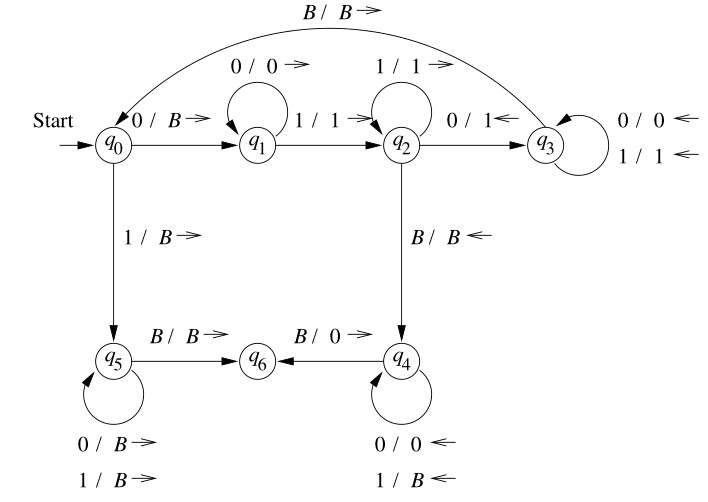
\includegraphics[width=0.7\textwidth]{files/tmta.PNG}
    \end{center}
    
    %$M=(\{q_0,q_1,q_2,q_3,q_4,q_5,q_6\},\{0,1\},\{0,1,B\},\delta,q_0,B)$    

    \vspace{-15pt}
    \begin{multicols}{2}
        $m,n$ encoded in unary\\
        at the start: $0^{m}10^n$\\
        at the end: $0^{m\frac{.}{\ } n}$\\
        find leftmost 0, delete\\
        search right for a 1\\
        if found, continue\\
        find a 0, rewrite by 1\\
        return left\\
        if no 0 found, either left or right:\\
        right: replace all 1s by B\\
        left ($m<n$): replace all 1s and 0s by B (leave the tape blank)      
    \end{multicols}

\end{frame}


\begin{frame}{Halting, recursively enumerable and recursive languages}
        
    \begin{definition}
        A TM \alert{halts} if it enters a state $q$, scanning a tape symbol $X$, and there is no transition in this situation, i.e., $\delta(q,X)$ is undefined.
    \end{definition}

    A TM halts whenever it gets to an accepting state (no outgoing transitions allowed). In general, we cannot require that a TM always halts, even if it does not accept.

    (Until a TM halts, we  do not know whether it will accept or not.)

    \smallskip

    \begin{definition}
        A language $L$ is:
        \begin{itemize}
            \item \alert{recursively enumerable} if it is recognized by some TM
            \item \alert{recursive} if there exists at TM $M$ that recognizes $L$ and \emph{halts on every input} $w\in\Sigma^*$
        \end{itemize}
    \end{definition}
  
\end{frame}


\begin{frame}{We will see that\dots}

    \begin{center}
        \Large
        context-sensitive $\subsetneq$ recursive $\subsetneq$ recursively enumerable $\subsetneq$ all languages
    \end{center}


    \begin{itemize}
        \item Every context-sensitive language is recursive.
        \item Not all recursive languages are context sensitive.
        \item Every recursive language is recursively enumerable.
        \item Not all recursively enumerable languages are recursive.
        \item A language is recursively enumerable, iff it is generated by a Type 0 grammar in the Chomsky hierarchy.
        \item Not all languages are recursively enumerable.   
    \end{itemize}

\end{frame}


\section{3.2 Variants of TMs}


\section*{Construction tricks}


\begin{frame}{Construction trick: storage in the FA unit}

    The following TM recognizes the language $L=01^*+10^*$; it remembers $0$, $1$, or $B$ in its state:
    $$d
    M=(\{q_0,q_1\}\times\{0,1,B\},\{0,1\},\{0,1,B\},\delta,[q_0,B],B,\{[q_1,B]\})
    $$
    \begin{center}
        \begin{tabular}{r |c |c |c }
        $\delta$ & 0 & 1 & B \\
        \hline\hline
        $\rightarrow[q_0,B]$& $([q_1,0],0,R)$& $([q_1,1],1,R)$& \\
        $[q_1,0]$& & $([q_1,0],1,R)$& $([q_1,B],B,R)$ \\
        $[q_1,1]$& $([q_1,1],0,R)$& &$([q_1,B],B,R)$ \\
        $*[q_1,B]$ & & &
        \end{tabular}
    \end{center}

    In general, we can store a finite number of variables with finitely many possible values (e.g. Boolean, input symbols, etc.): the state is a tuple, entries are values of the variables.
    
\end{frame}


\begin{frame}{Construction trick: tape with multiple tracks}

    To split the tape into two tracks, each of which can hold a tape symbol:
    $\Gamma'=\Gamma\cup\{\begin{smallmatrix}X\\Y\end{smallmatrix}\mid X,Y\in\Gamma\}$. At the beginning, traverse the input changing $a$ to $\begin{smallmatrix}B\\a\end{smallmatrix}$, then return.

    Or say $\Gamma=\{0,1,B\}$ and we want to put a mark $*$ over certain digits. Then $\Gamma'=\{0,1,B,\begin{smallmatrix}\phantom{*}\\0\end{smallmatrix},\begin{smallmatrix}*\\0\end{smallmatrix},\begin{smallmatrix}\phantom{*}\\1\end{smallmatrix},\begin{smallmatrix}*\\1\end{smallmatrix}\}$. (We write $[X,Y]$ for $\begin{smallmatrix}X\\Y\end{smallmatrix}$.)

    \begin{center}
        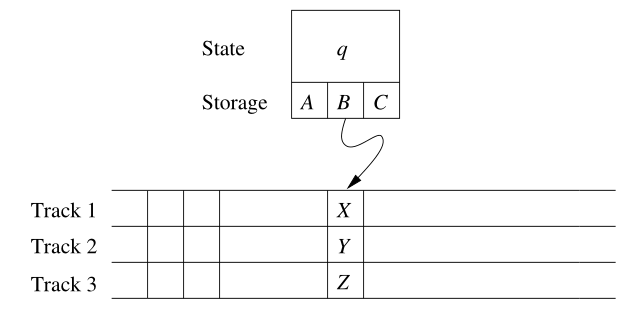
\includegraphics[width=0.6\textwidth]{files/tmmt.PNG}    
    \end{center}
    
    \textbf{NB:} This is different from (but will be used to simulate!) multiple tapes with heads moving independently. 
        
    
\end{frame}


\begin{frame}{Example: $L_{wcw}=\{wcw\mid w \in \{0,1\}^+\}$}

   
    Put a mark `$*$' over the letter being  checked, store it in memory. 
    (We skip the preprocessing, assume $a$ is already $[B,a]$.)

    $M=(\{q_0,\ldots,q_9\}\times\{0,1,B\},\{[B,0],[B,1],[B,c]\},\{B,*\}\times\{0,1,B,c\},\delta,[q_1,B],[B,B],\{[q_9,B]\})$ where $\delta$ is ($a,b\in\Sigma$):
    \begin{itemize}
        \item $\delta([q_1,B],[B,a])=([q_2,a],[*,a],R)$ pick up the symbol $a$
        \item $\delta([q_2,a],[B,b])=([q_2,a],[B,b],R)$ move right, search for $c$
        \item $\delta([q_2,a],[B,c])=([q_3,a],[B,c],R)$ continue right, state changed
        \item $\delta([q_3,a],[*,b])=([q_3,a],[*,b],R)$ continue right
        \item $\delta([q_3,a],[B,a])=([q_4,B],[*,a],L)$ match symbols, clear memory
        \item $\delta([q_4,B],[*,a])=([q_4,B],[*,a],L)$ go left
        \item $\delta([q_4,B],[B,c])=([q_5,B],[B,c],L)$ $c$ found, continue left
        \item are all symbols left and right checked? branch adequately\\
        \vdots
    \end{itemize}   

\end{frame}


\begin{frame}{Example continued}

    \begin{itemize}
        \item are all symbols left and right checked? branch adequately		
        \item $\delta([q_5,B],[B,a])=([q_6,B],[B,a],L)$  left symbol unchecked
        \item $\delta([q_6,B],[B,a])=([q_6,B],[B,a],L)$  proceed left
        \item $\delta([q_6,B],[*,a])=([q_1,B],[*,a],R)$  start again
        \item $\delta([q_5,B],[*,a])=([q_7,B],[*,a],R)$  symbol left from $c$ checked, go right
        \item $\delta([q_7,B],[B,c])=([q_8,B],[B,c],R)$  proceed right
        \item $\delta([q_8,B],[*,a])=([q_8,B],[*,a],R)$  proceed right
        \item $\delta([q_8,B],[B,B])=([q_8,B],[B,B],R)$  accept
    \end{itemize}
    
\end{frame}


\section*{Multi-tape Turing Machines}


\begin{frame}{A multi-tape TM}

    \begin{columns}

        \column{0.6\textwidth}

        \textbf{Initial configuration:}
        \begin{itemize}
            \item input on first tape, others blank
            \item first head scans the first input letter
            \item FA unit in the initial state
        \end{itemize}    
        \textbf{One step:}
        \begin{itemize}
            \item FA unit switches to the new state
            \item on each tape rewrite independently            
            \item each head moves independently
        \end{itemize}
        \mbox{\textbf{Transition function:} $\delta\colon(Q\setminus F)\times\Gamma^n\rightarrow Q\times \Gamma^n\times \{L,R\}^n$}
    
    
        \column{0.4\textwidth}
    
        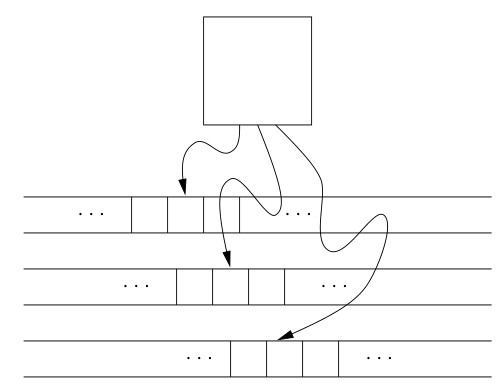
\includegraphics[width=1.1\textwidth]{files/tmmultitape.PNG}
        
    \end{columns}

    \bigskip

    \begin{theorem}
        Any language recognized by a multi-tape TM is also recognized by some (single-tape) Turing machine.
    \end{theorem}
    %(Note the difference between multi-track and multi-tape.)

\end{frame}


\begin{frame}{Proof: simulate using multiple tracks, mark head positions}

    \vspace{-6pt}
    \begin{flushright}
        \hspace{3cm}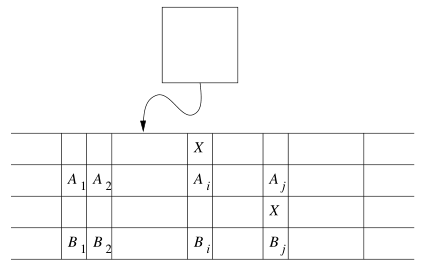
\includegraphics[width=0.48\textwidth]{files/tmmultitrack.PNG}    
    \end{flushright}
    
    \vspace{-3cm}
    Split the single tape into $2k$ tracks
    
    \begin{itemize}\setlength{\itemindent}{0pt}
        \item odd: mark $i^{th}$ head position
        \item even tracks: $i^{th}$ tape contents
    \end{itemize}

    \vspace{0.5cm}

    To simulate one step, visit all heads and store in the FA unit:
    \vspace{-6pt}       
    \begin{itemize}
        \item the simulated state
        \item the number of head marks to the left of us
        \item for every $i$, the symbol under $i^{th}$ head
    \end{itemize}

    Then we know enough to simulate one step. We visit all heads again to rewrite and move them.   \hfill\qedsymbol

        
    Simulating $n$ steps of a $k$-tape TM takes $O(n^2)$ moves. (One step takes $4n+2k$, heads no further than $2n$; read, write, move marks).

\end{frame}


\section*{Nondeterministic Turing Machines}


\begin{frame}{Nondeterministic Turing Machine}

    \begin{definition}
        A \alert{nondeterministic Turing machine} is $M=(Q,\Sigma, \Gamma, \delta,q_0,B,F)$ where $Q,\Sigma,\Gamma,q_0,B,F$ are the same as for a determ. TM, and
        \vspace{-3pt}
        $$
        \delta: (Q- F)\times \Gamma\rightarrow \mathcal P(Q\times\Gamma\times\{L,R\})
        $$
        \vspace{-18pt}
        
        A word $w\in \Sigma^*$ \alert{is accepted} by the nondeterminisic TM $M$ iff there exists an accepting sequence of moves $q_0w\vdash^* \alpha p \beta$, $p\in F$.
    \end{definition} 
    
    \begin{theorem}
        For every nondeterministic Turing machine $M_N$ there exist a deterministic TM $M_D$ such that $L(M_N)=L(M_D)$.
    \end{theorem}

    \textbf{Proof idea:} Subset construction not possible, the tape is infinite. Instead, BFS of the computation graph. In $k$ steps, at most $m^k$ configs for $m=\max_{q\in Q,x\in\Gamma} |\delta(q,x) |$. Store on a tape \& process.

\end{frame}


\begin{frame}{Proof}

    Breadth-first search of all possible computations of $M_N$ (configurations reachable from the initial configuration).

    Use a two-tape TM:
    \begin{itemize}
        \item \textbf{first tape:} maintain a queue of open vertices (configurations) separated by a special symbol
        \item \textbf{second tape:} scratch tape for processing one configuration
    \end{itemize}

    To process one configuration: 
	\begin{itemize}
        \item copy it to the scratch tape, dequeue (erase)
        \item read the state and scanned symbol
		\item if accepting state, accept and halt
		\item for each possible transition of $\delta_N$: perform the move and enqueue the resulting config (write at the end of tape 1)
	\end{itemize}
    \vspace{-6pt}
    [The transition function $\delta_N$ is encoded in $\delta_D$.]

\end{frame}


\begin{frame}{One-way infinite tape}

    \begin{theorem}
        Every recursively enumerable language is also recognized by a TM whose head never moves left of its initial position.
    \end{theorem}
        
    \medskip
    \begin{center}
        \begin{tabular}{|c|c|c|c}
        \hline
        $X_0$ &$X_1$ &$X_2$ & \ldots\hspace{5cm}\  \\ \hline
        * &$X_{-1}$ &$X_{-2}$ & \ldots \hspace{5cm}\ \\
        \hline
        \end{tabular}
    \end{center}
    \textbf{Proof idea:} Two-track tape, lower track for negative indices. Remember in state if positive or negative. If negative, $L$ means moving to the right and vice versa. Special cases around 0.\hfill\qedsymbol

    \bigskip

    \textbf{Exercise:} Consider a variant of Turing Machine with an infinite 2D board instead of a tape, moves $\{\uparrow,\rightarrow,\downarrow,\leftarrow\}$. Show how to simulate by the standard TM.
    
\end{frame}


\begin{frame}{Summary of Lecture 10}

    \begin{itemize}        
        \item Turing machine: two-way infinite tape, read, write, move head
        \item Accept iff in a final state; configurations
        \item TMs with output, computing a function
        \item Recursively enumerable vs. recursive languages (always halt).
        \item Construction tricks: 
        \begin{itemize}
            \item storage in state
            \item multiple tracks (on a single tape)
        \end{itemize}
        \item Variants of TMs: 
        \begin{itemize}
            \item multi-tape (independent heads),
            \item nondeterministic (accept iff some choices lead to final state)
        \end{itemize}  
    \end{itemize}
    
\end{frame}



\end{document}


